\RequirePackage{shellesc}
\immediate\write18{cd ..; tex spath3_code.dtx}
\documentclass{article}
\usepackage[svgnames]{xcolor}
\RequirePackage[enable-debug]{expl3}
\ExplSyntaxOn
\debug_on:n {check-declarations, deprecation}
\ExplSyntaxOff
\usepackage{tabularx}
\usepackage{tikz}
\usetikzlibrary{
  spath3,
  intersections,
  patterns,
  hobby}

\makeatletter
\def\showpath{%
  \def\pgfqpoint##1##2{(##1, ##2)}%
  \def\pgfsyssoftpath@movetotoken##1##2{%
    M\{##1\}\{##2\}
  }%
  \def\pgfsyssoftpath@linetotoken##1##2{%
    L\{##1\}\{##2\}
  }%
  \def\pgfsyssoftpath@curvetotoken##1##2{%
    C\{##1\}\{##2\}
  }%
  \def\pgfsyssoftpath@curvetosupportatoken##1##2{%
    Ca\{##1\}\{##2\}
  }%
  \def\pgfsyssoftpath@curvetosupportbtoken##1##2{%
    Cb\{##1\}\{##2\}
  }%
  \def\pgfsyssoftpath@closepathtoken##1##2{%
    Z\{##1\}\{##2\}
  }%
}
\makeatother

% Note: this was for a previous version and doesn't work with the
% current one, but it might be useful to adapt it to the current
% version so I'm keeping it around to remember what it originally
% looked like.

\newcommand\displaypath[1]{%

Displaying path information for: #1

\begin{tabularx}{\textwidth}{r@{:\hskip\arraycolsep}>{\raggedright\arraybackslash}X}
Length & \SPathInfo{#1}{length} \\
Real length & \SPathInfo{#1}{reallength} \\
Number of components & \SPathInfo{#1}{numberofcomponents} \\
Initial point & \showpath\SPathInfoInto{#1}{initialpoint}{\stuff}\expandafter\pgfqpoint\stuff \\
Final point & \showpath\SPathInfoInto{#1}{finalpoint}{\stuff}\expandafter\pgfqpoint\stuff \\
Initial action & \texttt{\showpath\SPathInfo{#1}{initialaction}} \\
Final action & \texttt{\showpath\SPathInfo{#1}{finalaction}} \\
Path & \texttt{\showpath\SPathInfo{#1}{path}} \\
Reverse path & \texttt{\showpath\SPathInfo{#1}{reversepath}} \\
Min bb & \showpath\SPathInfoInto{#1}{minbb}{\stuff}\expandafter\pgfqpoint\stuff \\
Max bb & \showpath\SPathInfoInto{#1}{maxbb}{\stuff}\expandafter\pgfqpoint\stuff 
\end{tabularx}%
}

\makeatletter
\tikzset{
  show last coords/.code={
    \edef\tikz@last@coords{(%
      \the\tikz@lastx,
      \the\tikz@lasty), (%
      \the\tikz@lastxsaved,
      \the\tikz@lastysaved), (%
      \the\tikz@lastmovetox,
      \the\tikz@lastmovetoy)%
    }%
    \show\tikz@last@coords
  },
  show tikz timer/.code={
    \show\tikz@timer
  }
}
\makeatother

\ExplSyntaxOn

\DeclareDocumentCommand\SPathPoint {m m}
{
  \spath_get_point_at:nnN {#1} {#2} \l__tmpa_tl
  \tl_show:N \l__tmpa_tl
}

\ExplSyntaxOff
\begin{document}

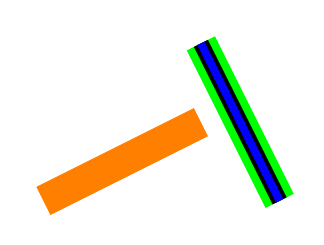
\begin{tikzpicture}
\path[spath/save=a] (0,0) -- (2,1);
\begin{scope}[xshift=3cm,rotate=90]
\draw[spath/use=a,orange,line width=4mm];
\draw[spath/use={a, transform={xshift=3cm, rotate=90}},green, line width=4mm];
\draw[spath/use={a,use current transformation},line width=2mm];
\draw[line width=1mm,blue] (0,0) -- (2,1);
\end{scope}
\end{tikzpicture}



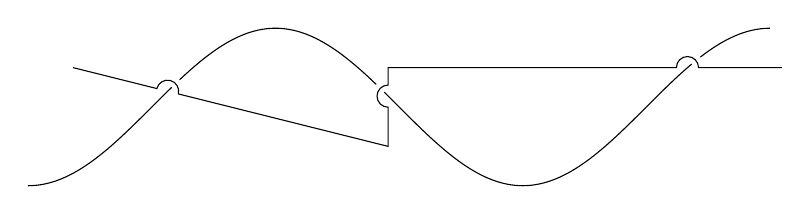
\begin{tikzpicture}
\coordinate (a) at (-1,0.5);
\coordinate (b) at (8,0.5);
\coordinate (c) at (3,-0.5);
\path[spath/save=sine]
(-1.57,-1)
cos ++(1.57,1)
sin ++(1.57,1)
cos ++(1.57,-1)
sin ++(1.57,-1)
cos ++(1.57,1)
sin ++(1.57,1);
\path[spath/save=over] (a) -- (c) |- (b);

\path[spath/save=arc] (0,0) arc[radius=1cm, start angle=180, delta angle=-180];

\tikzset{
  spath/split at intersections with={over}{sine},
  spath/insert gaps after components={over}{8pt},
  spath/join components upright with={over}{arc},
  spath/split at intersections with={sine}{over},
  spath/insert gaps after components={sine}{4pt},
}

\draw[spath/use=sine];
\draw[spath/use=over];
\end{tikzpicture}


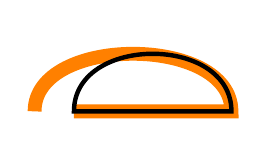
\begin{tikzpicture}
\draw[line width=5pt,orange] (0,0) -- (2,0) to[out=90,in=90] (-.5,0);
\draw[ultra thick] (0,0) -- (2,0) to[out=90,in=90] (-.5,0)
[spath/adjust and close=current]
;
\end{tikzpicture}


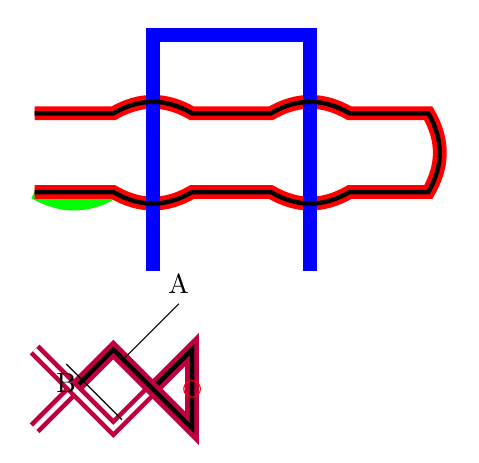
\begin{tikzpicture}
\path[spath/save=abc,draw=green, line width=5pt] (0,0) to[bend right] (1,0);
\path[spath/save=def,draw=red, line width=5pt]
  (0,0) -- ++(1,0)
++(1,0) -- ++(1,0)
++(1,0) -- ++(1,0)
++(0,1) -- ++(-1,0)
++(-1,0) -- ++(-1,0)
++(-1,0) -- ++(-1,0)
[
  spath/join components with={current}{abc},
]
;

\path[spath/save=ghi, draw, blue, line width=5pt] (1.5,-1) -- ++(0,3) -- ++(2,0) -- ++(0,-3);

\tikzset{
  spath/split at intersections={def}{ghi},
}

\draw[ultra thick, spath/use=def];

\path[spath/save=jkl, draw=purple, line width=5pt] (0,-3) -- ++(1,1) -- ++(1,-1) -- ++(0,1) -- ++(-1,-1) -- ++(-1,1);

\tikzset{
  spath/split at self intersections=jkl,
  spath/insert gaps after components={jkl}{5pt}{1,3},
  spath/join components={jkl}{3,5},
  spath/get components of={jkl}\Cpts
}

\tikzset{
  every jkl component/.style={draw, ultra thick},
  jkl component 1/.style={white},
  jkl component 3/.style={white},
  spath/render components=jkl
}

\draw[spath/transform to={jkl}{.25}] (0,0) -- +(0,1) node[above] {A};
\draw[spath/upright transform to={jkl}{.75}] (0,0) -- +(0,1) node[below] {B};

\draw[red] (spath cs:jkl .5) circle[radius=3pt];

\end{tikzpicture}



% Checking errors
\begin{tikzpicture}
\foreach \pth in {a,b,c,d,e,f,g,h,i,j,k,l,m,n,o,p,q,r,s,t,u,v,w,x,y,z}
{
  \path[spath/save=\pth] (0,0);
}
\foreach \pth in {A,B,C,D,E,F,G,H,I,J,K,L,M,N,O,P,Q,R,S,T,U,V,W,X,Y,Z}
{
  \path[spath/save=\pth] (0,0);
}

\tikzset{
  spath/.cd,
  clone=aA,
  clone global=bB,
  save to aux=c,
  export to svg=d,
  use=e,
  restore=f,
  restore reverse=g,
  append=h,
  append no move=i,
  append reverse=j,
  append reverse no move=k,
  insert=l,
  insert reverse=m,
  show=n,
  join with=oO,
  spot weld=p,
  spot weld globally=q,
  reverse=r,
  reverse globally=s,
  span=t{(0,0)}{(2,3)},
  span global=u{(0,0)}{(2,3)},
  splice=vVw,
  splice global=xXy,
  join components with=zZ,
  join components globally with=aA,
  join components upright with=bB,
  join components globally upright with=cC,
  close=d,
  close globally=e,
  close with=fF,
  close globally with=gG,
  shorten at end=h{5pt},
  shorten at start=i{5pt},
  shorten at both ends=j{5pt},
  shorten globally at end=k{5pt},
  shorten globally at start=l{5pt},
  shorten globally at both ends=m{5pt},
  translate=n{5pt}{5pt},
  translate globally=o{5pt}{5pt},
  normalise=p,
  normalise globally=q,
  transform=r{shift={(3,2)}},
  transform globally=s{shift={(3,2)}},
  split at intersections with=tT,
  split globally at intersections with=uU,
  split at intersections=vV,
  split globally at intersections=wW,
  split at self intersections=x,
  split globally at self intersections=y,
  get components of=z\cpts,
  get components of globally=a\cpts,
  render components=b,
  insert gaps after components=c{5pt},
  insert gaps globally after components=d{5pt},
  join components=e,
  join components globally=f,
  remove empty components=g,
  remove empty components globally=h,
  replace lines=i,
  replace lines globally=j,
  remove components=k{2},
  remove components globally=l{2},
  maybe spot weld=m,
  maybe spot weld globally=n,
  transform to=o{1.5},
  upright transform to=p{1.5},
}
\end{tikzpicture}

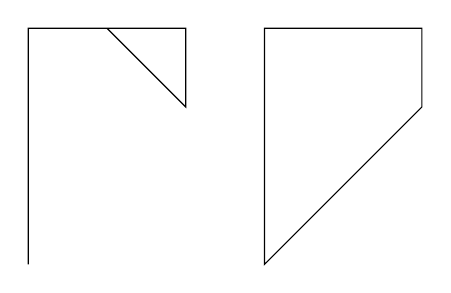
\begin{tikzpicture}

\path[spath/save=zig] (0,0) |- ++(1,1) +(0,0) -| ++(1,-1);

\draw (0,-2) -- ++(0,2) [spath/use={zig,weld}] -- cycle;

\path[spath/save=zag] (3,0) |- ++(1,1) -| ++(1,-1);

\draw (3,-2) -- ++(0,2) [spath/use={zag,weld}] -- cycle;
\end{tikzpicture}



\begin{tikzpicture}
\begin{scope}
\draw[spath/save=a] (0,0) -- +(2,0);
\end{scope}

\draw[spath/save=b] (0,-1) -- +(0,2);
\tikzset{
  spath/split at intersections with=ab
}
\end{tikzpicture}


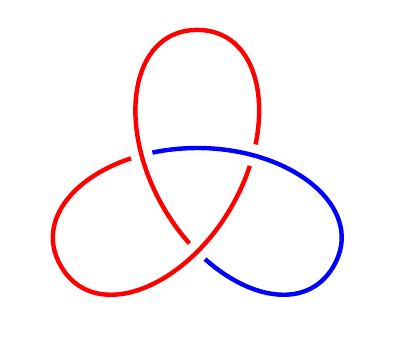
\begin{tikzpicture}[
  use Hobby shortcut,
  knot/.style 2 args={
    every #1 component/.style={ultra thick, draw, red},
    #1 component 1/.style={blue},
    spath/.cd,
    split at self intersections=#1,
    remove empty components=#1,
    insert gaps after components={#1}{8pt}{#2},
    spot weld=#1,
    render components=#1
  }
]
\path[spath/save=trefoil] ([closed]90:2) foreach \k in {1,...,3} { .. (-30+\k*240:.5) .. (90+\k*240:2) } (90:2);
\tikzset{knot={trefoil}{1,3,5}}
\end{tikzpicture}



\tikzset{
  test/.code 2 args={
    \message{Got: #1, #2}
  },
  test=abc,
  test={a}{b}{c},
  test={a}{bc}
}

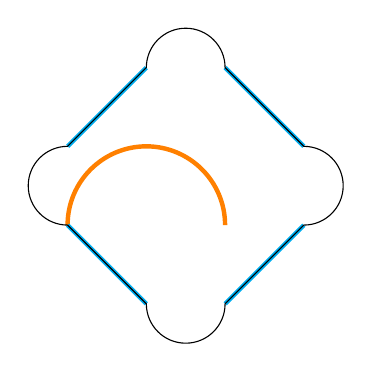
\begin{tikzpicture}
\path[
  draw=orange,
  ultra thick,
  spath/save=arc] (0,0) arc[radius=1,start angle=180, end angle=0];

\path[
  draw=cyan,
  ultra thick,
  spath/save=start]
(0,1) -- ++(1,1)
++(1,0) -- ++(1,-1)
++(0,-1) -- ++(-1,-1)
++(-1,0) -- ++(-1,1)
;

\tikzset{
  spath/join components with={start}{arc},
  spath/close with={start}{arc},
}

\draw[spath/restore=start];
\end{tikzpicture}

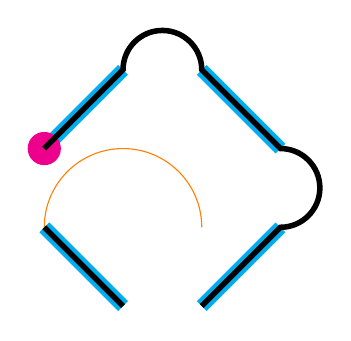
\begin{tikzpicture}
\path[
  draw=orange,
  spath/save=arc] (0,0) arc[radius=1,start angle=180, end angle=0];

\path[
  draw=cyan,
  line width=5pt,
  spath/save=start]
(0,1) -- ++(1,1)
++(1,0) -- ++(1,-1)
++(0,-1) -- ++(-1,-1)
++(-1,0) -- ++(-1,1)
;

\fill[magenta]
(0,1) circle[radius=6pt]
;

\tikzset{
  spath/join components with={start}{arc}{1,2},
}

\draw[line width=2pt, spath/restore=start];
\end{tikzpicture}




\begin{tikzpicture}
\path[spath/save=ab] (0,0) to[out=0,in=180] +(3,1);
\path[spath/save=cd] (0,2) to[out=90,in=-90] +(3,1);
\tikzset{
  spath/join with={ab}{cd, reverse, move, weld, transform={scale=2,rotate=90}},
  spath/show=ab,
}
\draw[
  orange,
  ultra thick,
  spath/restore=ab
];
\end{tikzpicture}


\begin{tikzpicture}[scale=2]
\path[spath/save=ab] (0,1) -- ++(2,0);
\draw[spath/restore=ab] node[auto,pos=.5] {ab} node[auto,pos=.75] {bc};
\draw[spath/transform={ab}{scale=3},spath/restore=ab] node[auto,pos=.5] {ab};
\end{tikzpicture}


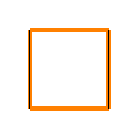
\begin{tikzpicture}
\draw[orange, ultra thick, spath/save=sq]
(0,0) -- ++(1,0)
+(0,0) -- ++(0,1)
+(0,0) -- ++(-1,0)
+(0,0) -- ++(0,-1)
;

\tikzset{
  spath/remove components={sq}{1,3},
  spath/show=sq
}

\draw[spath/restore=sq];
\end{tikzpicture}


\begin{tikzpicture}
\path[draw=orange,ultra thick,spath/save=a] (3,2) -- ++(1,1) to[out=90,in=-90] ++(3,0);

\tikzset{
  spath/span={a}{(4,5)}{(7,1)}
}

\fill
(4,5) circle[radius=3pt]
(7,1) circle[radius=3pt]
;

\draw[spath/restore=a];

\draw (0,0) -- +(1,0) to[spath/to={a}] node[pos=.6,auto] {node} ++(2,-1) -- +(0,1);
\fill
(0,0) circle[radius=3pt]
+(1,0) circle[radius=3pt]
++(2,-1) circle[radius=3pt]
+(0,1) circle[radius=3pt]
;
\end{tikzpicture}

\begin{tikzpicture}
\path[draw=orange,ultra thick,spath/save=a] (3,2) -- ++(1,1) to[out=90,in=-90] ++(3,0);
\tikzset{
  spath/show=a,
  spath/normalise=a,
  spath/show=a,
}

\draw[spath/transform={a}{scale=28},spath/restore=a];
\end{tikzpicture}


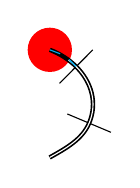
\begin{tikzpicture}
\fill[red]  (0.01869pt, 54.94537pt) circle[radius=8pt];


\draw[ultra thick,spath/save=short]
(-0.05162pt, 16.03508pt)
.. controls (5.78798pt, 19.31158pt)
and (11.75685pt, 22.57562pt)
.. (14.22594pt, 28.45274pt)
.. controls (17.33452pt, 35.85257pt)
and (15.03658pt, 43.39893pt)
.. (9.5325pt, 48.87686pt)
.. controls (6.97835pt, 51.41888pt)
and (3.73378pt, 53.5155pt)
.. (0.01869pt, 54.94537pt)
;

\draw[spath/transform to={short}{.3333}] (0,0) +(0,.3) -- +(0,-.3);
\draw[spath/transform to={short}{.6666}] (0,0) +(0,.3) -- +(0,-.3);

\draw[white,
  spath/shorten at end={short}{8pt},
  spath/show=short,
  spath/restore=short];

\draw[cyan] (0.01869pt, 54.94537pt) --
 (3.73378pt, 53.5155pt)
(9.5325pt, 48.87686pt)
-- (6.97835pt, 51.41888pt)
  ;

\end{tikzpicture}


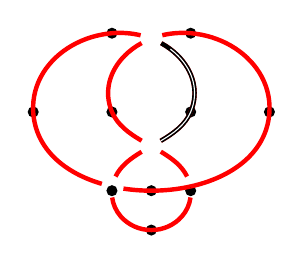
\begin{tikzpicture}[
  every spath component/.style={ultra thick, draw, red},
  use Hobby shortcut,
]
\path[spath/save=figure8] ([closed]0,0) .. (1.5,1) .. (.5,2) .. (-.5,1) .. (.5,0) .. (0,-.5) .. (-.5,0) .. (.5,1) .. (-.5,2) .. (-1.5,1) .. (0,0);
\fill (0,0) circle[radius=2pt]
 (1.5,1) circle[radius=2pt]
 (.5,2) circle[radius=2pt]
 (-.5,1) circle[radius=2pt]
 (.5,0) circle[radius=2pt]
 (0,-.5) circle[radius=2pt]
 (-.5,0) circle[radius=2pt]
 (.5,1) circle[radius=2pt]
 (-.5,2) circle[radius=2pt]
 (-1.5,1) circle[radius=2pt]
;
\tikzset{
  spath/draft mode=true,
  spath/knot={figure8}{8pt}{},%2,4,6,8},
  spath/get components of={figure8}\cpts,
  spath/show=\getComponentOf\cpts{6},
  spath/insert gaps after components={figure8}{8pt}{6},
  spath/get components of={figure8}\ncpts,
  spath/show=\getComponentOf\ncpts{6},
}
\draw[ultra thick,spath/restore=\getComponentOf\cpts{6}];
\draw[white,spath/restore=\getComponentOf\ncpts{6}];
\path (0,-.7);
\end{tikzpicture}


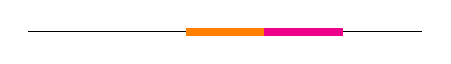
\begin{tikzpicture}
\path[spath/save=g,draw]
(0,0) -- ++(1,0)
++(0,0) -- ++(1,0)
++(0,0) -- ++(1,0)
++(0,0) -- ++(1,0)
++(0,0) -- ++(1,0)
;
\tikzset{spath/get components of={g}\cpts}

\draw[line width=3pt, orange, spath/restore=\getComponentOf{\cpts}{3}];
\draw[line width=3pt, magenta, spath/restore=\getComponentOf{\cpts}{4}];
\end{tikzpicture}


\begin{tikzpicture}
\path[spath/save=a] (0,0) -- node[pos=.5,auto] {\(a\)}
 ++(2,0) to[out=0,in=-90] node[pos=.5,auto] {\(b\)} ++(2,2) to[out=90,in=0] node[pos=.5,auto] {\(c\)} ++(-2,2)
;
\draw[spath/restore=a]
node[pos=.16,auto,swap] {\(a\)}
node[pos=.5,auto,swap,sloped] {\(b\)}
node[pos=.84,auto,swap,sloped,allow upside down] {\(c\)}
;

\draw (0,-1) -- ++(3,-1) [spath/append=a]
node[pos=.16,auto,swap] {\(a\)}
node[pos=.5,auto,swap,sloped] {\(b\)}
node[pos=.84,auto,swap,sloped,allow upside down] {\(c\)}
;
\end{tikzpicture}


\begin{tikzpicture}
\begin{scope}[scale=.5, rotate=30, xscale=2, shift={(3,-1)}]
\path
(0,0) node[circle,fill] {}
(2,1) node[circle,fill] {}
++(2,0) node[circle,fill] {}
+(0,1) node[circle,fill] {}
+(0,3) node[circle,fill] {}
+(1,0) node[circle,fill] {}
;
\draw[spath/save global=b, line width=5pt, orange] (2,1) -- ++(1,1) -- +(1,-1) [show last coords];
\end{scope}
\path
(spath cs:b 1) node[circle,fill=blue] {}
+(0,1) node[circle,fill=blue] {}
+(0,3) node[circle,fill=blue] {}
+(1,0) node[circle,fill=blue] {}
;

\tikzset{spath/show=b}
\draw[spath/restore=b,show last coords] -- +(0,1);
\tikzset{spath/show=b}
\begin{scope}[scale=3]
\draw[spath/restore=b,show last coords] -- +(0,1);
\end{scope}
\draw[spath/restore=b] to[out=-90,in=-90] +(1,0);
\draw[spath/restore=b] to[out=-90,in=-90] cycle;
\end{tikzpicture}


\begin{tikzpicture}[use Hobby shortcut]
\path[spath/save=figure8] ([closed]0,0) .. (1.5,1) .. (.5,2) .. (-.5,1) .. (.5,0) .. (0,-.5) .. (-.5,0) .. (.5,1) .. (-.5,2) .. (-1.5,1) .. (0,0);
\tikzset{spath/knot={figure8}{8pt}{2,4,6,8}}
\path (0,-.7);
\end{tikzpicture}


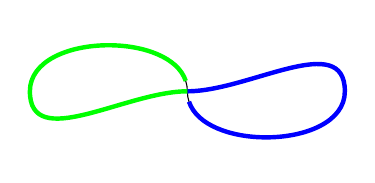
\begin{tikzpicture}
\path[spath/save=curve,draw] (0,0) to[out=-90,in=180] (2,0) to[out=0,in=90] (4,0) to[out=-90,in=-90] (2,0) to[out=90,in=90] cycle;
\tikzset{
  every spath component/.style={draw, ultra thick},
  curve component 1/.style={blue},
  curve component 2/.style={green},
  curve component 3/.style={orange},
  curve component 4/.style={magenta},
  curve component 5/.style={cyan},
  curve component 6/.style={green!50!black},
  curve component 7/.style={yellow!50!black},
  curve component 8/.style={red!50!black},
  curve component 9/.style={blue!50!black},
  spath/draft mode=true,
  spath/knot={curve}{8pt}{},
}
\end{tikzpicture}

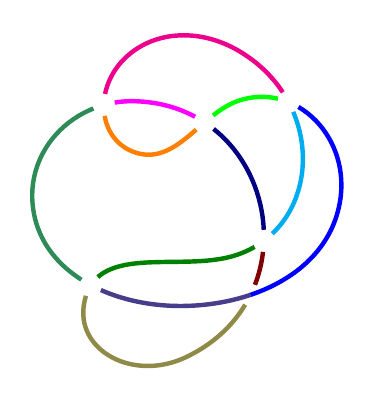
\begin{tikzpicture}[use Hobby shortcut]
\path[spath/save=6-3,scale=1.3] ([closed]0,0) .. (1.5,1) .. (.5,2) .. (-.5,1.5) .. (-.5,2.5) .. (.5,2.5) .. (.5,.5) .. (-1,0) .. (0,-.5) .. (-.5,2) .. (-1.5,1) .. (0,0);
\tikzset{
  every spath component/.style={draw,ultra thick},
  6-3 component 1/.style={blue},
  6-3 component 2/.style={green},
  6-3 component 3/.style={orange},
  6-3 component 4/.style={magenta},
  6-3 component 5/.style={cyan},
  6-3 component 6/.style={green!50!black},
  6-3 component 7/.style={yellow!50!black},
  6-3 component 8/.style={red!50!black},
  6-3 component 9/.style={blue!50!black},
  6-3 component 10/.style={Fuchsia},
  6-3 component 11/.style={SeaGreen},
  6-3 component 12/.style={DarkSlateBlue},
  spath/draft mode=true,
  spath/knot={6-3}{8pt}{},%2,4,...,12}
}
\end{tikzpicture}


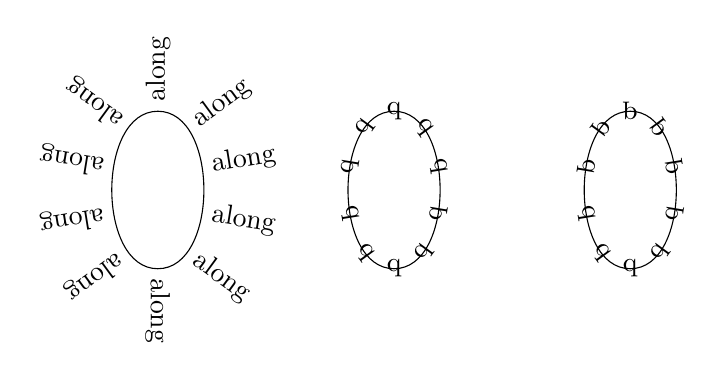
\begin{tikzpicture}
\draw[spath/save=oval] (0,0) to[out=0,in=0] (0,2) to[out=180,in=180] (0,0);
\foreach \k in {0,...,9} {
  \node[transform shape, allow upside down=false, spath/transform to={oval}{0.\k}, rotate=-90,right] {along};
}
\begin{scope}[xshift = 3cm]
\draw[spath/save=soval] (0,0) to[out=0,in=0] (0,2) to[out=180,in=180] (0,0);
\foreach \k in {0,...,9} {
  \node[transform shape, spath/upright transform to={soval}{0.\k}] {q};
}
\begin{scope}[xshift = 3cm]
\draw[spath/save=soval] (0,0) to[out=0,in=0] (0,2) to[out=180,in=180] (0,0);
\foreach \k in {0,...,9} {
  \node[transform shape, spath/transform to={soval}{0.\k}] {q};
}
\end{scope}
\end{scope}
\end{tikzpicture}



\begin{tikzpicture}
\draw[spath/save=oval] (0,0) to[out=0,in=0] (0,2) +(-1,0) to[out=180,in=180] (0,0);
\tikzset{spath/spot weld=oval}
\end{tikzpicture}

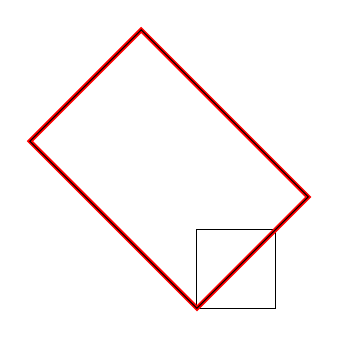
\begin{tikzpicture}
\draw[spath/save=tpath] (0,0) rectangle +(1,1);
\draw[rotate=45, xscale=2, yscale=3, ultra thick, red] (0,0) rectangle +(1,1);
\draw[
  spath/transform={tpath}{rotate=45, xscale=2, yscale=3},
  spath/restore={tpath}];
\end{tikzpicture}

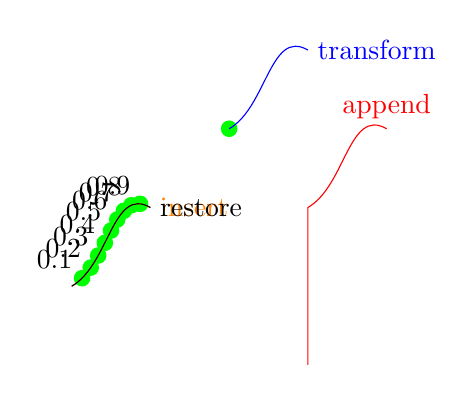
\begin{tikzpicture}
\path[spath/save=rpath] (0,0) to[out=30,in=150] (1,1);
\foreach \k in {1,...,9} {
  \fill[green] (spath cs:rpath 0.\k) circle[radius=3pt];
  \node[above left] at (spath cs:rpath 0.\k) {\(0.\k\)};
}
\fill[green] (2,2) circle[radius=3pt];
\draw[blue, spath/transform={rpath}{shift={(2,2)}}, spath/restore={rpath}] node[right] {transform};
\draw[orange] (3,0) [spath/insert={rpath}] node[right] {insert};
\draw[red] (3,-1) -- +(0,2) [spath/append={rpath}] node[above] {append};
\draw[spath/restore={rpath}] node[right] {restore};
\end{tikzpicture}

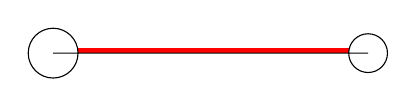
\begin{tikzpicture}
\path[spath/save=apath] (0,0) foreach \k in {1,...,4} { -- ++(1,0) +(0,0)};
\draw[
  spath/shorten at end={apath}{7pt},
  spath/shorten at start={apath}{9pt},
  spath/translate={apath}{0pt}{1pt},
  spath/restore=apath,
  ultra thick, red
];
\draw (0,0) circle[radius=9pt] [spath/insert=apath] circle[radius=7pt];
\end{tikzpicture}

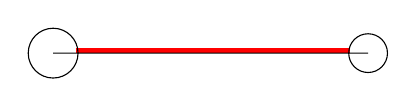
\begin{tikzpicture}
\path[spath/save=apath] (0,0) foreach \k in {1,...,4} { to[out=0,in=180] ++(1,0) +(0,0)};
\draw[
  ultra thick,
  red,
  spath/.cd,
  shorten at end={apath}{7pt},
  shorten at start={apath}{9pt},
  translate={apath}{0pt}{1pt},
  restore=apath,
];
\draw (0,0) circle[radius=9pt] [spath/insert=apath] circle[radius=7pt];
\end{tikzpicture}

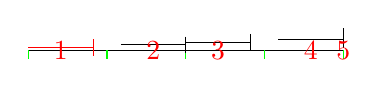
\begin{tikzpicture}
\draw[spath/save=npath] (0,0) foreach \k in {1,...,4} { -- ++(1,0) +(0,0)};
\draw[green] (0,0) -- +(0,-3pt) foreach \k in {1,...,4} { -- +(0,-3pt) ++(1,0)} -- +(0,-3pt);
%\expandafter\show\csname tikz@intersect@path@name@npath\endcsname
\tikzset{
  spath/.cd,
  insert gaps after components={npath}{10pt}{1,3},
  get components of={npath}\components,
}
%\show\components

\tikzset{
  path 1/.style={
    red,
  },
}

\foreach[count=\k] \cpt in \components {
  \path[
    draw,
    path \k/.try,
    spath/.cd,
    translate=\cpt{0pt}{\k pt},
    restore=\cpt,
  ] +(0,3pt) -- +(0,-3pt);
  \node[text=red] at (spath cs:{\cpt} .5) {\(\k\)};
}
\end{tikzpicture}

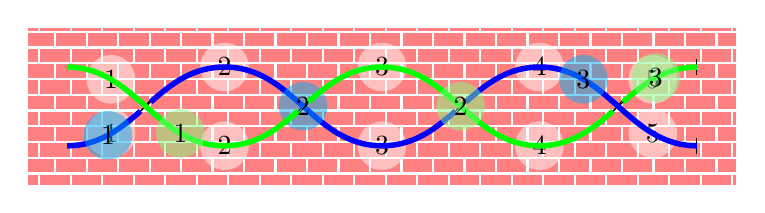
\begin{tikzpicture}[
  use Hobby shortcut,
]

\fill[red!50!white] (-.5,-.5) rectangle (8.5,1.5);
\fill[pattern=bricks, pattern color=white] (-.5,-.5) rectangle (8.5,1.5);

\path[spath/save=pathA] (0,0) to[out=0,in=180] ++(2,1) to[out=0,in=180] ++(2,-1)  to[out=0,in=180] ++(2,1)  to[out=0,in=180] ++(2,-1);
\path[spath/save=pathB] (0,1) to[out=0,in=180] ++(2,-1) to[out=0,in=180] ++(2,1)  to[out=0,in=180] ++(2,-1)  to[out=0,in=180] ++(2,1);

\tikzset{
  spath/.cd,
  split at intersections={pathA}{pathB},
  get components of={pathA}\pathAcomponents,
  get components of={pathB}\pathBcomponents,
}

\foreach[count=\k] \cpt in \pathAcomponents {
  \draw[spath/restore=\cpt,-|];
  \node[fill=white, fill opacity=.5, circle, text opacity=1] at (spath cs:{\cpt} .5) {\(\k\)};
}

\foreach[count=\k] \cpt in \pathBcomponents {
  \draw[spath/restore=\cpt,-|];
  \node[fill=white, fill opacity=.5, circle, text opacity=1] at (spath cs:{\cpt} .5) {\(\k\)};
}

\tikzset{
  spath/.cd,
  insert gaps after components={pathA}{5pt}{1,3},
  join components={pathA}{3,5},
  get components of={pathA}\pathAcomponents,
  insert gaps after components={pathB}{5pt}{2,4},
  join components={pathB}{2,4},
  get components of={pathB}\pathBcomponents,
}

\foreach[count=\k] \cpt in \pathAcomponents {
  \draw[blue, line width=2pt,spath/restore=\cpt];
  \node[fill=cyan, fill opacity=.5, circle, text opacity=1] at (spath cs:{\cpt} .5) {\(\k\)};
}

\foreach[count=\k] \cpt in \pathBcomponents {
  \draw[green, line width=2pt,spath/restore=\cpt];
  \node[fill=green!50, fill opacity=.5, circle, text opacity=1] at (spath cs:{\cpt} .5) {\(\k\)};
}
\end{tikzpicture}

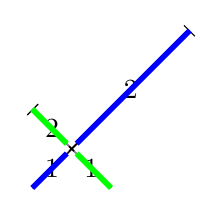
\begin{tikzpicture}
\draw[spath/save=pathA] (0,0) -- (2,2);
\draw[spath/save=pathB] (1,0) -- (0,1);

\tikzset{
  spath/.cd,
  split at intersections={pathA}{pathB},
  get components of={pathA}\pathAcomponents,
  get components of={pathB}\pathBcomponents,
}

\foreach[count=\k] \cpt in \pathAcomponents {
  \draw[spath/restore=\cpt,-|];
  \node[fill=white, fill opacity=.5, circle, text opacity=1] at (spath cs:{\cpt} .5) {\(\k\)};
}

\foreach[count=\k] \cpt in \pathBcomponents {
  \draw[spath/restore=\cpt,-|];
  \node[fill=white, fill opacity=.5, circle, text opacity=1] at (spath cs:{\cpt} .5) {\(\k\)};
}

\tikzset{
  spath/.cd,
  insert gaps after components={pathA}{5pt}{1},
  get components of={pathA}\pathAcomponents,
  insert gaps after components={pathB}{5pt}{1},
  get components of={pathB}\pathBcomponents,
}

\foreach[count=\k] \cpt in \pathAcomponents {
  \draw[blue, line width=2pt,spath/restore=\cpt];
%  \node[fill=cyan, fill opacity=.5, circle, text opacity=1] at (spath cs:{\cpt} .5) {\(\k\)};
}

\foreach[count=\k] \cpt in \pathBcomponents {
  \draw[green, line width=2pt,spath/restore=\cpt];
%  \node[fill=cyan, fill opacity=.5, circle, text opacity=1] at (spath cs:{\cpt} .5) {\(\k\)};
}


\end{tikzpicture}

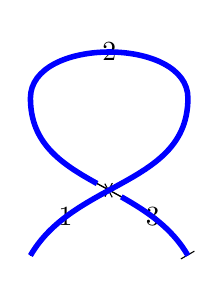
\begin{tikzpicture}
\draw[
  scale=2,
  spath/save=npath,
] (0,0) to[out=60,in=-90] (1,1) to[out=90,in=90] (0,1) to[out=-90,in=120] (1,0);

\tikzset{
  spath/.cd,
  split at self intersections=npath,
  get components of={npath}\npathcomponents,
}

\foreach[count=\k] \cpt in \npathcomponents {
  \draw[spath/restore=\cpt,-|];
  \node[fill=white, fill opacity=.5, circle, text opacity=1] at (spath cs:{\cpt} .5) {\(\k\)};
}

\tikzset{
  spath/.cd,
  insert gaps after components={npath}{10pt}{2},
   join components={npath}{2},
  get components of={npath}\npathcomponents,
}

\foreach[count=\k] \cpt in \npathcomponents {
  \draw[blue, line width=2pt,spath/restore=\cpt];
%  \node[fill=cyan, fill opacity=.5, circle, text opacity=1] at (spath cs:{\cpt} .5) {\(\k\)};
}

\end{tikzpicture}

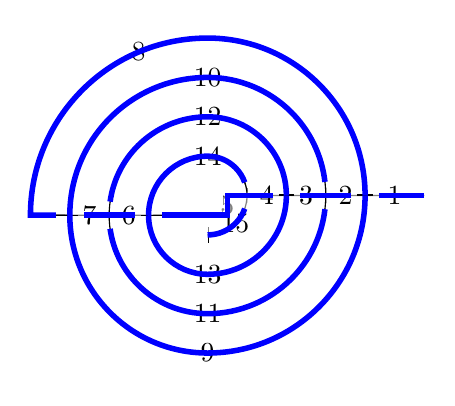
\begin{tikzpicture}
\draw[spath/save=line] (5,0) -- (2.5,0) -- ++(0,-.25) -- ++(-2.5,0)
arc[radius=2.25cm,start angle=180,end angle=90]
arc[radius=2cm,start angle=90, delta angle=-180]
arc[radius=1.75cm,start angle=-90, delta angle=-180]
arc[radius=1.5cm,start angle=90, delta angle=-180]
arc[radius=1.25cm,start angle=-90, delta angle=-180]
arc[radius=1cm,start angle=90, delta angle=-180]
arc[radius=.75cm,start angle=-90, delta angle=-180]
arc[radius=.5cm,start angle=90, delta angle=-180]
;

\tikzset{
  spath/.cd,
  split at self intersections=line,
  get components of={line}\pathcomponents,
}

\foreach[count=\k] \cpt in \pathcomponents {
  \draw[spath/restore=\cpt,-|];
  \node[fill=white, fill opacity=.5, circle, text opacity=1] at (spath cs:{\cpt} .5) {\(\k\)};
}


\tikzset{
  spath/.cd,
  insert gaps after components={line}{10pt}{1,3,5,7,10,11,14},
%  join components={line}{2,4,6,8,9,12,13},
  get components of={line}\pathcomponents,
}

\foreach[count=\k] \cpt in \pathcomponents {
  \draw[blue, line width=2pt,spath/restore=\cpt];
%  \node[fill=cyan, fill opacity=.5, circle, text opacity=1] at (spath cs:{\cpt} .5) {\(\k\)};
}


\end{tikzpicture}


\end{document}
